\section{Sketching}
The structure can look like this:
\begin{itemize}
	\item Present the chosen design challenges and some of the initial concerns in the beginning phase
	\item Each challenge is outlined with:
		\begin{itemize}
			\item Sketches
			\item Design thoughts for the sketch - what was the thought behind this sketch?
			\item summary of the group discussion for this case - what worked, what didn't and why?
		\end{itemize}
	\item Conclude what the final sketches are - what do they accomplish, and what do they lack(maybe reference what might be discussed in future work)?
\end{itemize}
\subsection{How do we access the application? (Menu)}
The menu is an essential part of any application. It outlines the possibilities for the user in a simple fashion. The menu is something every user has experience with, as it is the first thing a user is met with when running an application. This means that the menu has to contain of certain classic elements.\par A user needs a way to close the application. On mobile phones nowadays this can be done with 'return' buttons on the phone, but all applications generally have a built in exit function.\par
The user also needs to have some sort of options menu, and guidelines. This is a must for this application. Stacking LEGO seems simple and intuitive, but all the operations and possibilities is something that can confuse a potential user. \par
Lastly the menu needs to have an easy access to the LEGO session itself. It shouldn't be complicated for the user to start a new LEGO session, meaning that this action should be as intuitive as it gets.\par
\begin{center}
	Insert sketch 1:
\end{center}

\subsection{The main menu screen}
The initial ideas for the main menu were generated following the 'x plus x' sketch generation principle outlined in the course. In the case of the sketching done for the main menu, a '5 plus 5' scheme was used. One common theme in the sketching of the main menu was separation of the design of the menu and the interaction with the menu, and the difficulties with making that separation. In quite a few of the earlier sketches, what was being sketched was more a way of interacting with the menu rather than the design of the menu itself.

\subsection{The generator board}
After discussing menus in the context of the Hololens, it became apparent that there was a need for a menu that could be placed and interacted with in the real world. Using the tracking capabilities of the Hololens, different designs of the so called 'generator board' came up. The main purpose of the generator board is to generate blocks that the user can then drag out of the predefined spawning space.\\
\\
The idea came up that a menu with the same look and functionality of a tablet device could make interaction second nature for the user. Having the ability to pick up, move and place the menu on a surface like a table or the floor seemed like a natural way of approaching the problem. The idea can be seen in a very early sketch in figure (HVILKEN FIGUR?):\\

\begin{figure}[H]
    \centering
    \begin{subfigure}[b]{0.5\textwidth}
        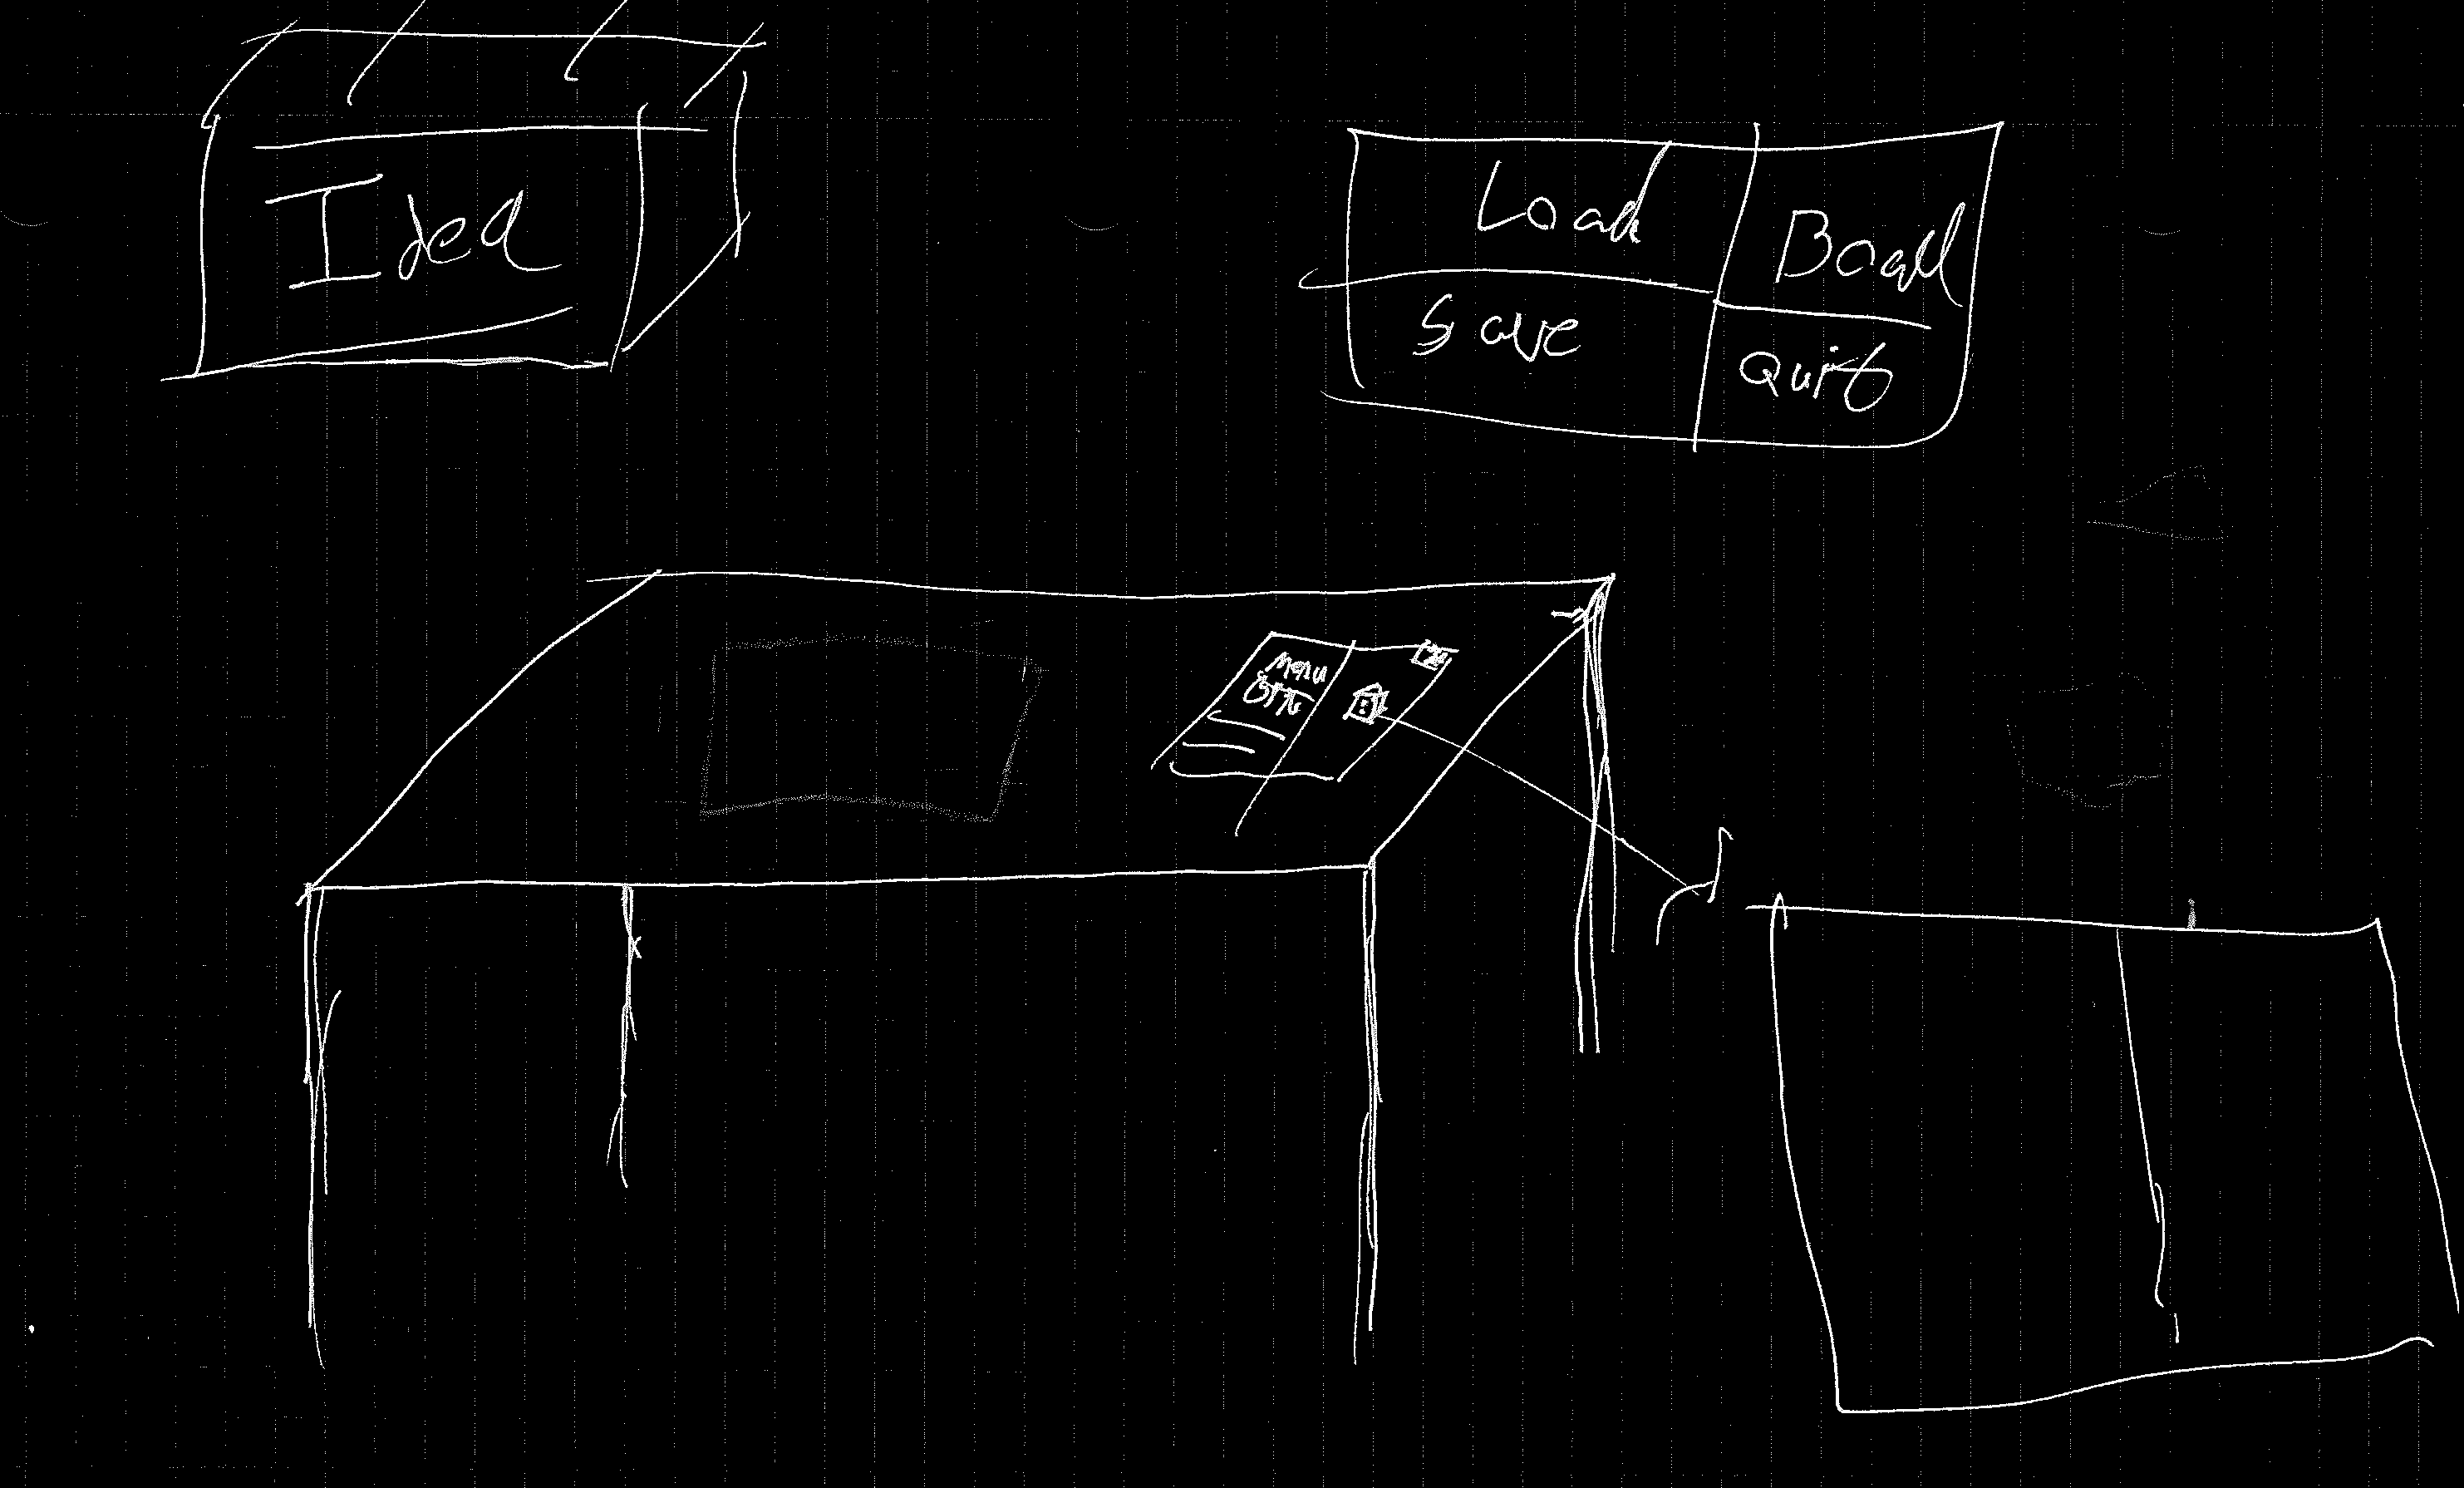
\includegraphics[width=\textwidth]{figures/Generator/gen6.png}
        \caption{Early sketch of the generator board as a 'tablet' on a table.}
    \end{subfigure}
    \caption{Excercise 1.5}
\end{figure}
